\documentclass[usenames,dvipsnames,tikz]{standalone}
\usetikzlibrary{shapes.geometric}
%\usepackage{xcolor}
\colorlet{tBlue}{RoyalBlue!35!Cerulean}
\colorlet{tRed}{Red}
%\usepackage{tikz}
%\usepackage{standalone}
\begin{document}
	
% SUB-MSCPP THRESHOLD GRAPH
	
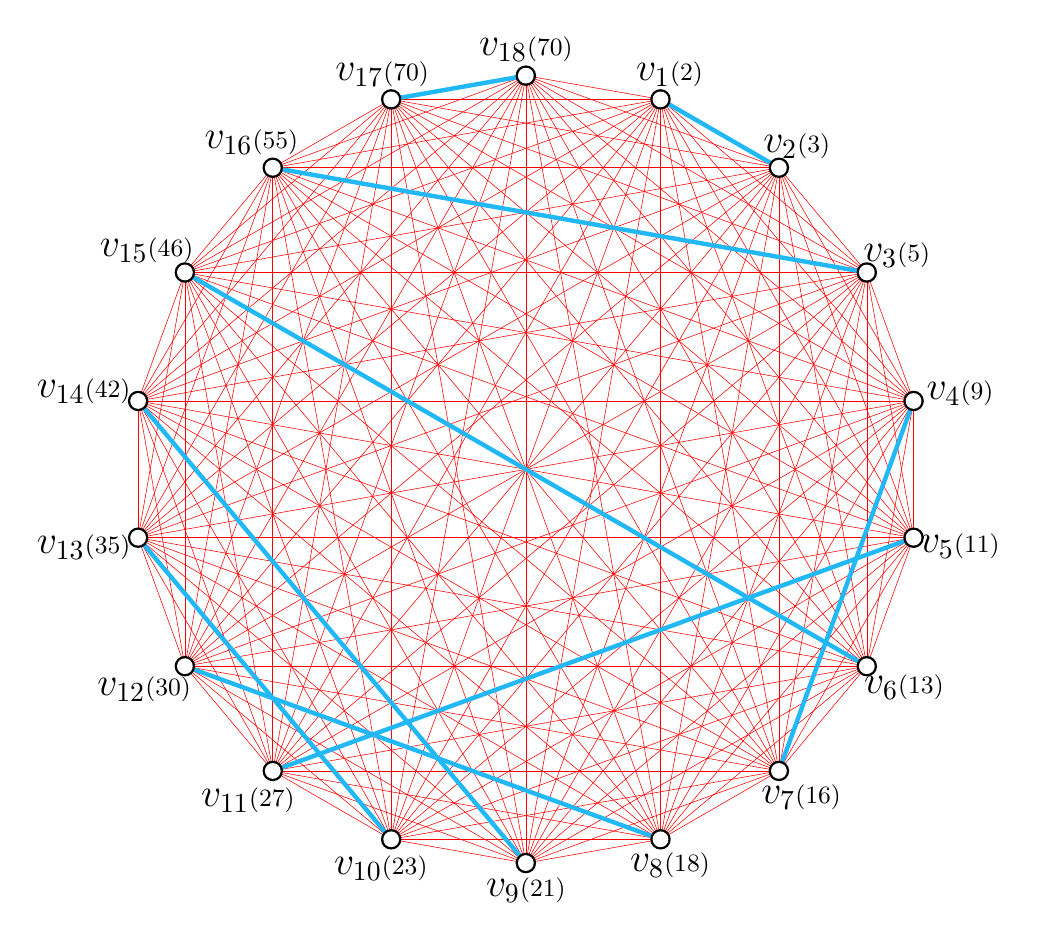
\begin{tikzpicture}
%Values of vertices:
% v1=2, v2=3, v3=5, v4=9, v5=11, v6=13, v7=16, v8=18, v9=21, v10=23, v11=27, v12=30, v13=35, v14=42, v15=46, v16=55, v17=70, v18=70 (v17/v18 universal vertices), \tau = 70.

%partners: v1-v2, v3-v16, v4-v7, v5-v11, v6-v15, v8-v12, v9-v14, v10-v13, v17-v18.


\foreach \n/\value in {1/1, 2/1, 3/2, 4/2, 5/3, 6/4, 7/4, 8/5, 9/5, 10/6, 11/6, 12/6, 13/6, 14/7, 15/8, 16/9, 17/10, 18/10}
	\fill (90-\n*20:5cm) coordinate (v\n) circle [radius = 0.1];
	
\foreach \n/\value in {1/2, 17/70, 18/70}
	\fill (90-\n*20:5cm) coordinate (v\n) circle [radius = 0.1]
		++(90-\n*20:9.5pt) node {\Large{$v_{\n}$}\small{($\value$)}};

\foreach \n/\value in {2/3, 8/18, 9/21}
	\fill (90-\n*20:5cm) coordinate (v\n) circle [radius = 0.1]
		++(90-\n*20:10pt) node {\Large{$v_{\n}$}\small{($\value$)}};
		
\foreach \n/\value in {3/5, 7/16}
	\fill (90-\n*20:5cm) coordinate (v\n) circle [radius = 0.1]
		++(90-\n*20:12.5pt) node {\Large{$v_{\n}$}\small{($\value$)}};		
		
\foreach \n/\value in {4/9, 5/11, 12/30}
	\fill (90-\n*20:5cm) coordinate (v\n) circle [radius = 0.1]
		++(90-\n*20:17pt) node {\Large{$v_{\n}$}\small{($\value$)}};

\foreach \n/\value in {15/46}
	\fill (90-\n*20:5cm) coordinate (v\n) circle [radius = 0.1]
		++(90-\n*20:16pt) node {\Large{$v_{\n}$}\small{($\value$)}};
	
\foreach \n/\value in {6/13}
	\fill (90-\n*20:5cm) coordinate (v\n) circle [radius = 0.1]
		++(90-\n*20:15.5pt) node {\Large{$v_{\n}$}\small{($\value$)}};
		
\foreach \n/\value in {10/23}
	\fill (90-\n*20:5cm) coordinate (v\n) circle [radius = 0.1]
		++(90-\n*20:11pt) node {\Large{$v_{\n}$}\small{($\value$)}};
		
\foreach \n/\value in {11/27}
	\fill (90-\n*20:5cm) coordinate (v\n) circle [radius = 0.1]
		++(90-\n*20:14pt) node {\Large{$v_{\n}$}\small{($\value$)}};
		
\foreach \n/\value in {13/35, 14/42}
	\fill (90-\n*20:5cm) coordinate (v\n) circle [radius = 0.1]
		++(90-\n*20:20pt) node {\Large{$v_{\n}$}\small{($\value$)}};	

\foreach \n/\value in {16/55}
	\fill (90-\n*20:5cm) coordinate (v\n) circle [radius = 0.1]
		++(90-\n*20:12pt) node {\Large{$v_{\n}$}\small{($\value$)}};	
	
	
%Edges and vertices
\foreach \m/\n in {1/3, 1/4, 1/5, 1/6, 1/7, 1/8, 1/9, 1/10, 1/11, 1/12, 1/13, 1/14, 1/15, 1/16, 1/17, 1/18, 2/3, 2/4, 2/5, 2/6, 2/7, 2/8, 2/9, 2/10, 2/11, 2/12, 2/13, 2/14, 2/15, 2/16, 2/17, 2/18, 3/4, 3/5, 3/6, 3/7, 3/8, 3/9, 3/10, 3/11, 3/12, 3/13, 3/14, 3/15, 3/17, 3/18, 4/5, 4/6, 4/8, 4/9, 4/10, 4/11, 4/12, 4/13, 4/14, 4/15, 4/16, 4/17, 4/18, 5/6, 5/7, 5/8, 5/9, 5/10, 5/12, 5/13, 5/14, 5/15, 5/16, 5/17, 5/18, 6/7, 6/8, 6/9, 6/10, 6/11, 6/12, 6/13, 6/14, 6/16, 6/17, 6/18, 7/8, 7/9, 7/10, 7/11, 7/12, 7/13, 7/14, 7/15, 7/16, 7/17, 7/18, 8/9, 8/10, 8/11, 8/13, 8/14, 8/15, 8/16, 8/17, 8/18, 9/10, 9/11, 9/12, 9/13, 9/15, 9/16, 9/17, 9/18, 10/11, 10/12, 10/14, 10/15, 10/16, 10/17, 10/18, 11/12, 11/13, 11/14, 11/15, 11/16, 11/17, 11/18, 12/13, 12/14, 12/15, 12/16, 12/17, 12/18, 13/14, 13/15, 13/16, 13/17, 13/18, 14/15, 14/16, 14/17, 14/18, 15/16, 15/17, 15/18, 16/17, 16/18}
	\draw [tRed, very thin] (v\n) -- (v\m);
\foreach \m/\n in {1/2, 3/16, 4/7, 5/11, 6/15, 8/12, 9/14, 10/13, 17/18}
	\draw [ultra thick, tBlue] (v\n) -- (v\m);
\foreach \n in {1,...,18}
	\fill (90-\n*20:5cm) coordinate (v\n) circle [radius = 0.13];
\foreach \n in {1,...,18}
	\fill [white] (90-\n*20:5cm) coordinate (v\n) circle [radius = 0.1];

\end{tikzpicture}
	
\end{document}